% Figure "wp_count" of "Galashin's Conjecture 4.3 via a convex gradient": the cycle count of the winding-one partitions
% (eq. for |Z|; CLH-5), for the two partitions A and B of the worked window, as bars of cyclic advance.
% Source in the paper's own fonts at the text width (6.5in = 468bp). It adds no assertion.
% Every value drawn is read from Lean output lines (SHA-256 of the lines):
%   picture D99  0f70644c8492e5a7757e876cfb1217f30b695e80672fadfc43805abb6dd320d5   (partition A)
%   picture D100 f674297b2a22ae1df8436116e6b95677cb2e5ad68cf3796567f235ad26c02165   (partition B)
%   crossP = Conj43.crossEdges of the window (3,5,1,2,4), in paper labels
% Advances and wraps are integer counts made in Lean over the partitions' cycles.
% Build: pdflatex <this file> && pdftocairo -svg <this file>.pdf <this file>.svg
\documentclass[11pt]{standalone}
\usepackage[T1]{fontenc}
\usepackage{lmodern}
\usepackage{amsmath,amssymb}
\usepackage{tikz}
\usetikzlibrary{arrows.meta,positioning,calc}

% the palette of the paper's other figures: blue solid for the first strand, cycle or arc, ochre dashed for the second
\definecolor{ink}{HTML}{233740}
\definecolor{muted}{HTML}{65757D}
\definecolor{pblue}{HTML}{0072B2}
\definecolor{qochre}{HTML}{B87827}

\tikzset{
  base/.style={draw=muted, line width=0.5pt},
  ttl/.style={font=\small, text=ink, inner sep=0pt},
  lab/.style={font=\footnotesize, inner sep=1.2pt, text=ink},
  labm/.style={font=\small, inner sep=1.2pt, text=ink},
  labP/.style={font=\small, inner sep=1.2pt, text=pblue},
  labQ/.style={font=\small, inner sep=1.2pt, text=qochre},
  idx/.style={font=\footnotesize, text=muted, inner sep=0pt},
  negE/.style={font=\small, text=pblue, inner sep=0pt},
  posE/.style={font=\small, text=qochre, inner sep=0pt},
  zeroE/.style={font=\small, text=muted, inner sep=0pt},
  vtx/.style={circle, draw=ink, fill=white, line width=0.6pt, inner sep=0pt, minimum size=16bp, font=\small, text=ink},
  cycP/.style={pblue, line width=1.1pt, -{Stealth[length=5pt,width=4.2pt]}, shorten >=1pt, shorten <=1pt},
  cycQ/.style={qochre, line width=1.1pt, dash pattern=on 4pt off 1.6pt, -{Stealth[length=5pt,width=4.2pt]}, shorten >=1pt, shorten <=1pt},
  chord/.style={pblue, line width=0.9pt},
  arrP/.style={pblue, line width=1.0pt, -{Stealth[length=4.4pt,width=3.8pt]}},
  arrQ/.style={qochre, line width=1.0pt, dash pattern=on 4pt off 1.6pt, -{Stealth[length=4.4pt,width=3.8pt]}},
  arrM/.style={muted, line width=0.6pt, -{Stealth[length=4pt,width=3.4pt]}},
}

\begin{document}
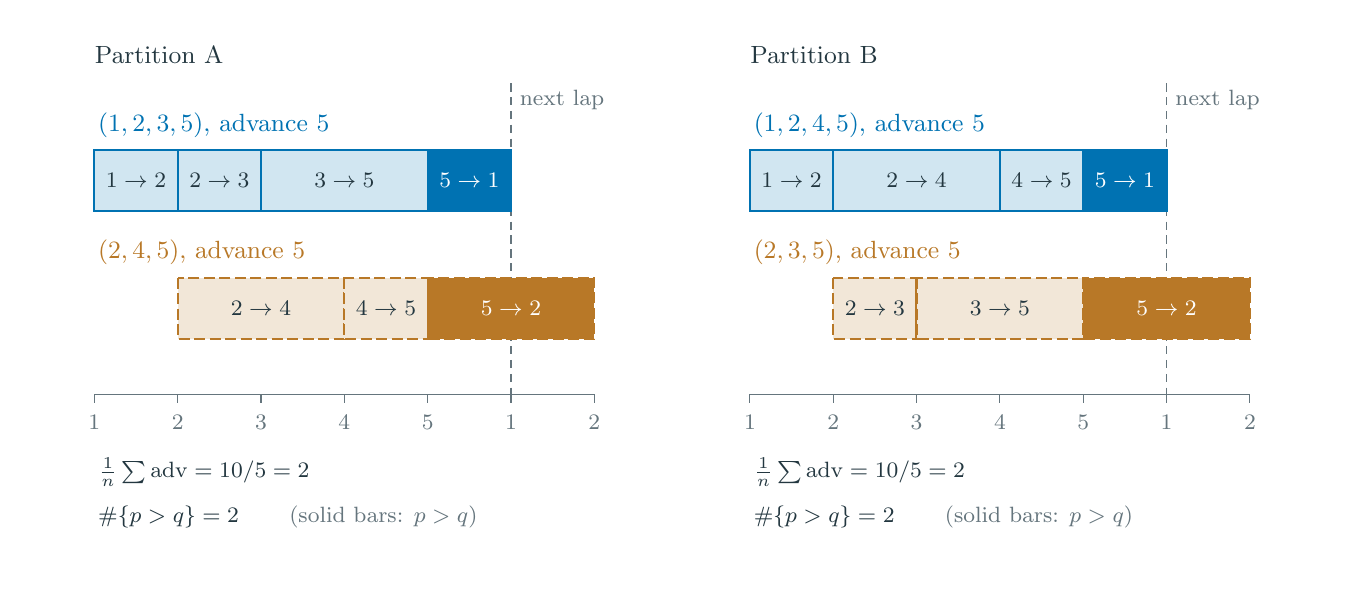
\begin{tikzpicture}[x=1bp,y=1bp]
\useasboundingbox (0,0) rectangle (468.000,192.000); %@ wp canvas w=468.000 h=192.000
\draw[muted, dash pattern=on 3pt off 2pt, line width=0.5pt] (174.000,172.000) -- (174.000,60.000); %@ wp A lap x=174.000
\node[ttl,anchor=west] at (24.000,182.000) {Partition A};
\node[labP,anchor=west] at (24.000,157.000) {$(1,2,3,5)$, advance $5$}; %@ wp A cycle=1,2,3,5 adv=5
\path[fill=pblue!18, draw=pblue, line width=0.8pt] (24.000,148.000) rectangle (54.000,126.000); %@ wp A seg cycle=1,2,3,5 p=1 q=2 start=0 adv=1 wrap=0 x0=24.000 x1=54.000
\node[lab,text=ink] at (39.000,137.000) {$1\to2$};
\path[fill=pblue!18, draw=pblue, line width=0.8pt] (54.000,148.000) rectangle (84.000,126.000); %@ wp A seg cycle=1,2,3,5 p=2 q=3 start=1 adv=1 wrap=0 x0=54.000 x1=84.000
\node[lab,text=ink] at (69.000,137.000) {$2\to3$};
\path[fill=pblue!18, draw=pblue, line width=0.8pt] (84.000,148.000) rectangle (144.000,126.000); %@ wp A seg cycle=1,2,3,5 p=3 q=5 start=2 adv=2 wrap=0 x0=84.000 x1=144.000
\node[lab,text=ink] at (114.000,137.000) {$3\to5$};
\path[fill=pblue, draw=pblue, line width=0.8pt] (144.000,148.000) rectangle (174.000,126.000); %@ wp A seg cycle=1,2,3,5 p=5 q=1 start=4 adv=1 wrap=1 x0=144.000 x1=174.000
\node[lab,text=white] at (159.000,137.000) {$5\to1$};
\node[labQ,anchor=west] at (24.000,111.000) {$(2,4,5)$, advance $5$}; %@ wp A cycle=2,4,5 adv=5
\path[fill=qochre!18, draw=qochre, line width=0.8pt, dash pattern=on 4pt off 1.6pt] (54.000,102.000) rectangle (114.000,80.000); %@ wp A seg cycle=2,4,5 p=2 q=4 start=1 adv=2 wrap=0 x0=54.000 x1=114.000
\node[lab,text=ink] at (84.000,91.000) {$2\to4$};
\path[fill=qochre!18, draw=qochre, line width=0.8pt, dash pattern=on 4pt off 1.6pt] (114.000,102.000) rectangle (144.000,80.000); %@ wp A seg cycle=2,4,5 p=4 q=5 start=3 adv=1 wrap=0 x0=114.000 x1=144.000
\node[lab,text=ink] at (129.000,91.000) {$4\to5$};
\path[fill=qochre, draw=qochre, line width=0.8pt, dash pattern=on 4pt off 1.6pt] (144.000,102.000) rectangle (204.000,80.000); %@ wp A seg cycle=2,4,5 p=5 q=2 start=4 adv=2 wrap=1 x0=144.000 x1=204.000
\node[lab,text=white] at (174.000,91.000) {$5\to2$};
\draw[muted, line width=0.4pt] (24.000,60.000) -- (204.000,60.000);
\draw[muted, line width=0.4pt] (24.000,60.000) -- (24.000,57.000);
\node[idx] at (24.000,50.000) {$1$}; %@ wp A tick pos=0 label=1
\draw[muted, line width=0.4pt] (54.000,60.000) -- (54.000,57.000);
\node[idx] at (54.000,50.000) {$2$}; %@ wp A tick pos=1 label=2
\draw[muted, line width=0.4pt] (84.000,60.000) -- (84.000,57.000);
\node[idx] at (84.000,50.000) {$3$}; %@ wp A tick pos=2 label=3
\draw[muted, line width=0.4pt] (114.000,60.000) -- (114.000,57.000);
\node[idx] at (114.000,50.000) {$4$}; %@ wp A tick pos=3 label=4
\draw[muted, line width=0.4pt] (144.000,60.000) -- (144.000,57.000);
\node[idx] at (144.000,50.000) {$5$}; %@ wp A tick pos=4 label=5
\draw[muted, line width=0.4pt] (174.000,60.000) -- (174.000,57.000);
\node[idx] at (174.000,50.000) {$1$}; %@ wp A tick pos=5 label=1
\draw[muted, line width=0.4pt] (204.000,60.000) -- (204.000,57.000);
\node[idx] at (204.000,50.000) {$2$}; %@ wp A tick pos=6 label=2
\node[idx,anchor=west] at (177.000,166.000) {next lap};
\node[lab,anchor=west] at (24.000,32.000) {$\tfrac1n\sum\operatorname{adv}=10/5=2$}; %@ wp A total=10 n=5 count=2
\node[lab,anchor=west] at (24.000,16.000) {$\#\{p>q\}=2$}; %@ wp A wraps=2
\node[idx,anchor=west] at (94.000,16.000) {(solid bars: $p>q$)};
\draw[muted, dash pattern=on 3pt off 2pt, line width=0.5pt] (410.000,172.000) -- (410.000,60.000); %@ wp B lap x=410.000
\node[ttl,anchor=west] at (260.000,182.000) {Partition B};
\node[labP,anchor=west] at (260.000,157.000) {$(1,2,4,5)$, advance $5$}; %@ wp B cycle=1,2,4,5 adv=5
\path[fill=pblue!18, draw=pblue, line width=0.8pt] (260.000,148.000) rectangle (290.000,126.000); %@ wp B seg cycle=1,2,4,5 p=1 q=2 start=0 adv=1 wrap=0 x0=260.000 x1=290.000
\node[lab,text=ink] at (275.000,137.000) {$1\to2$};
\path[fill=pblue!18, draw=pblue, line width=0.8pt] (290.000,148.000) rectangle (350.000,126.000); %@ wp B seg cycle=1,2,4,5 p=2 q=4 start=1 adv=2 wrap=0 x0=290.000 x1=350.000
\node[lab,text=ink] at (320.000,137.000) {$2\to4$};
\path[fill=pblue!18, draw=pblue, line width=0.8pt] (350.000,148.000) rectangle (380.000,126.000); %@ wp B seg cycle=1,2,4,5 p=4 q=5 start=3 adv=1 wrap=0 x0=350.000 x1=380.000
\node[lab,text=ink] at (365.000,137.000) {$4\to5$};
\path[fill=pblue, draw=pblue, line width=0.8pt] (380.000,148.000) rectangle (410.000,126.000); %@ wp B seg cycle=1,2,4,5 p=5 q=1 start=4 adv=1 wrap=1 x0=380.000 x1=410.000
\node[lab,text=white] at (395.000,137.000) {$5\to1$};
\node[labQ,anchor=west] at (260.000,111.000) {$(2,3,5)$, advance $5$}; %@ wp B cycle=2,3,5 adv=5
\path[fill=qochre!18, draw=qochre, line width=0.8pt, dash pattern=on 4pt off 1.6pt] (290.000,102.000) rectangle (320.000,80.000); %@ wp B seg cycle=2,3,5 p=2 q=3 start=1 adv=1 wrap=0 x0=290.000 x1=320.000
\node[lab,text=ink] at (305.000,91.000) {$2\to3$};
\path[fill=qochre!18, draw=qochre, line width=0.8pt, dash pattern=on 4pt off 1.6pt] (320.000,102.000) rectangle (380.000,80.000); %@ wp B seg cycle=2,3,5 p=3 q=5 start=2 adv=2 wrap=0 x0=320.000 x1=380.000
\node[lab,text=ink] at (350.000,91.000) {$3\to5$};
\path[fill=qochre, draw=qochre, line width=0.8pt, dash pattern=on 4pt off 1.6pt] (380.000,102.000) rectangle (440.000,80.000); %@ wp B seg cycle=2,3,5 p=5 q=2 start=4 adv=2 wrap=1 x0=380.000 x1=440.000
\node[lab,text=white] at (410.000,91.000) {$5\to2$};
\draw[muted, line width=0.4pt] (260.000,60.000) -- (440.000,60.000);
\draw[muted, line width=0.4pt] (260.000,60.000) -- (260.000,57.000);
\node[idx] at (260.000,50.000) {$1$}; %@ wp B tick pos=0 label=1
\draw[muted, line width=0.4pt] (290.000,60.000) -- (290.000,57.000);
\node[idx] at (290.000,50.000) {$2$}; %@ wp B tick pos=1 label=2
\draw[muted, line width=0.4pt] (320.000,60.000) -- (320.000,57.000);
\node[idx] at (320.000,50.000) {$3$}; %@ wp B tick pos=2 label=3
\draw[muted, line width=0.4pt] (350.000,60.000) -- (350.000,57.000);
\node[idx] at (350.000,50.000) {$4$}; %@ wp B tick pos=3 label=4
\draw[muted, line width=0.4pt] (380.000,60.000) -- (380.000,57.000);
\node[idx] at (380.000,50.000) {$5$}; %@ wp B tick pos=4 label=5
\draw[muted, line width=0.4pt] (410.000,60.000) -- (410.000,57.000);
\node[idx] at (410.000,50.000) {$1$}; %@ wp B tick pos=5 label=1
\draw[muted, line width=0.4pt] (440.000,60.000) -- (440.000,57.000);
\node[idx] at (440.000,50.000) {$2$}; %@ wp B tick pos=6 label=2
\node[idx,anchor=west] at (413.000,166.000) {next lap};
\node[lab,anchor=west] at (260.000,32.000) {$\tfrac1n\sum\operatorname{adv}=10/5=2$}; %@ wp B total=10 n=5 count=2
\node[lab,anchor=west] at (260.000,16.000) {$\#\{p>q\}=2$}; %@ wp B wraps=2
\node[idx,anchor=west] at (330.000,16.000) {(solid bars: $p>q$)};
\end{tikzpicture}
\end{document}
